\chapter{Laser-solid-plasma interaction: overview}\label{chapter:Laser-solid-plasma interaction: overview}
\minitoc

\thispagestyle{empty}

\section{Laser absorption in plasmas}
\label{sec:LaserAbsorptions}

In the early 70's efforts to control thermodynamical reactions using pellet targets\cite{nuckolls1972laser}, unusual surface absorption of the intense pulse light was observed experimentally \cite{self1976lawrence,brueckner1974laser,priedhorsky1981hard}, which was a hint that new nonlinear phenomena where taking place. The invoked mechanism to describe these observations was historically called ``resonant absorption'': the laser propagates in the underdense region of the solid density plasma  surface and reaches a regime called ``wavebreaking''. Here, strong coupling between the laser field and the plasma waves becomes possible. The authors who described this mechanism did not mention the possibility of high-order harmonic generation in the process, but did state that this could explain hot-electron acceleration from solid plasma targets \cite{freidberg1972resonant,albritton1975cold}. This was critical because this hot electron population would preheat the core of the pellet. In the 1993, Tabak~\cite{tabak1994ignition} proposed a fast ignition scheme where those same hot electrons were chosen to trigger nuclear reactions after an adiabatic compression, which is why their emission properties have to be controlled (low divergence, monoenergetic).\\
 In this chapter, we go over the physical concepts of the ``resonant absorption'' model, and highlight the different hypotheses made in order for it to be valid, among which that the plasma scale length should be ``long''. In his famous article called ``not-so-resonant, resonant absorption'' \cite{Brunel1987}, Brunel proposed a model, which we trivially call ``Brunel model'', more applicable in the case of short plasma scale lengths, as described in~\ref{section:Brunel absorption mechanism}.
%: the laser periodically excites electron at the plasma surface. When the laser force is oriented towards the plasma bulk, electrons can propagate deep enough to escape the screened laser field leading to a loss in laser energy (conversion to kinetic energy) . In addition to explain unsually laser absorption, this mechanism will prove to be essential in the modelisation of Coherent Wake Emission harmonics inside the plasma as described further in Chap? . 





\subsection{Resonant absorption}

To go over the basic principles of what is generaly called "resonant absorption", we will start by writing Maxwell's equations for both the magnetic and electric field in a plasma we assume to be non-magnetic ($\g{M}=\g{0}$) and non polar ($\g{P}=\g{0}$). These equations can be found in Appendix~\ref{ch:Normalisation conventions}.

\begin{subequations}
\label{eq:EandBequations}
\begin{align}[left = \empheqlbrace\,]
&\nabla^2 \g{E}(\g{r},t)  - \nabla ( \nabla. \g{E})  - \frac{1}{c^2} \partial_{t}^2 \g{E}(\g{r},t)  -\mu_0\partial_t \g{j}(\g{r},t) = \g{0}  \label{eq:Eequations}\\
&\nabla^2 \g{B}(\g{r},t) - \frac{1}{c^2}\partial_{t}^2 \g{B}(\g{r},t)  + \mu_0\nabla \times \g{j}(\g{r},t) =\g{0} \label{eq:Bequations} 
\end{align}
\end{subequations}

\noindent To close this system of equations, one needs to make a hypothesis about the response of the current $\g{j}$ to an electromagnetic field. We therefore suppose that the plasma of initial electronic density $n_{e0}$ is neutral, and that only the electrons (as opposed to the much heavier ions) are in motion. Moreover, we consider a ``cold'' plasma, which means we study its dynamics on a time scale where collisions can be neglected in the equation of motion. With those conditions met, we can use the non-relativistic equation of motion known for one electron and retrieve the expression of the current using the relation:
$$
\g{j}(r,t) = -en_e(\g{r},t) v_e(\g{r},t)
$$

\subsection{Neutral plasma response equations}

We suppose that the plasma density is independent of time $n_e(\g{r},t) = n_{e0}(\g{r})$. The function $n_{e0}(.)$ is often chosen to be exponentially decreasing towards vacuum as explained further in Chap~\ref{ch:Measuring the gradient expansion}. However, we do not need to make such a hypotheses within the scope of the present derivation.\\
The neutrality of the plasma is imposed at all time, which yields $\nabla \g{j}(\g{r},t) = 0$ because of the charge conservation. The dynamics of the system are described by the non-relativistic equation of motion ($\gamma =1$ and $\g{B}=\g{0}$, as described in Appendix~\ref{ch:Normalisation conventions})

\begin{equation}
\frac{d\g{v}_e}{dt}=\partial_t\g{v}_e + (\g{v}_e\nabla )\g{v}_e = -\frac{e}{m_e}\g{E}(r,t) 
\label{eq:EquationOfMotionNR}
\end{equation}

\noindent To linearize Eq.~\ref{eq:EquationOfMotionNR}, we make the assumption that $v_e<<L \omega_0$ where $L$ is the characteristic scale length of the problem and $\omega_0$ the driving laser frequency. Note that in a homogeneous plasma, $L$ is equal to the driving laser wavelength and that condition is automatically verified, but for strongly inhomogeneous plasmas however, $L$ can be significantly smaller. Assuming the inequality holds true, we have for a monochromatic field:

\begin{subequations}
\label{eq:Jderivation}
\begin{align}[left = \empheqlbrace\,]
&\g{j}(\g{r},\omega) = - n_{e0}(\g{r})\frac{e^2}{i\omega m_e}\g{E}(\g{r},\omega)  \label{eq:PartialJ} \\
&\nabla \times \g{j}(\g{r},\omega) = \frac{-e^2}{i\omega m_e}[\nabla n_{e0} \times \g{E}(\g{r},\omega)+n_{e0} i\omega\g{ B}(\g{r},\omega) ]\label{eq:NablaJ} 
\end{align}
\end{subequations}

\noindent We define:
$$
\omega_p(\g{r})^2 = \frac{n_{e0}(\g{r})e^2}{m_e\epsilon_0}
$$


\noindent By applying the $\nabla.$ operator to the \textit{Maxwell-Ampere} Equation given in ~\ref{eq:Maxwell-Equations}, it is easy to show that $\nabla j =0$ implies $\partial_t (\nabla E) = 0$.
Therefore, supposing the plasma was neutral at time $t=0$, this leads to $\nabla E = 0$ at all times in Eq.~\ref{eq:Eequations}. The
\textit{Maxwell-Ampere} equation in the Fourier domain also gives the relation:

\begin{equation}
\label{eq:Bfield}
\nabla \times \g{B} = \frac{ic^2\omega}{\omega^2-\omega_p(\g{r})^2}\g{E}(\g{r},\omega)
\end{equation}

\noindent  By injecting Eq.~\ref{eq:Bfield}  in Eq.~\ref{eq:EandBequations} and using the relations in~\ref{eq:Jderivation}, we obtain separate equations for $\g{E}$ and $\g{B}$, which are the equations commonly used to propagate the field undergoing ``resonant'' absorption in a plasma:



\begin{subequations}
\label{eq:RAequations}
\begin{align}[left = \empheqlbrace\,]
     &\nabla^2 \g{E}(\g{r},\omega) +  \frac{\omega^2-\omega_p(\g{r})^2}{c^2}\g{E}(\g{r},\omega)=0 \label{eq:RAequations1}\\
     &\nabla^2 \g{B}(\g{r},\omega) - \frac{1}{\omega^2-\omega_p(\g{r})^2}\nabla \omega_p^2 \times \nabla\times \g{B}+ \frac{\omega^2-\omega_p(\g{r})^2}{c^2} \g{B}(\g{r},\omega) =0 \label{eq:RAequations2}
\end{align}
\end{subequations}

\noindent Equation ~\ref{eq:RAequations1} shows the impossibility for the electric field to propagate for $\omega < \omega_p(\g{r})$ (this index is negative, as for a metallic mirror) which defines the \underline{critical surface equation}:
$$
n_e(\g{r})=n_c
$$ 

\noindent Above the critical surface, the electric field gets reflected and below, it becomes evanescent.

\subsection{Geometrical representation of resonant absorption}

Since resonant absorption applies to long gradient scale lengths, it is quite easy to confuse with the geometrical optics picture of a wave curving its $k$ vector along propagation as shown in Fig~\ref{fig:gradient}.

\begin{figure}[H]
\begin{center}
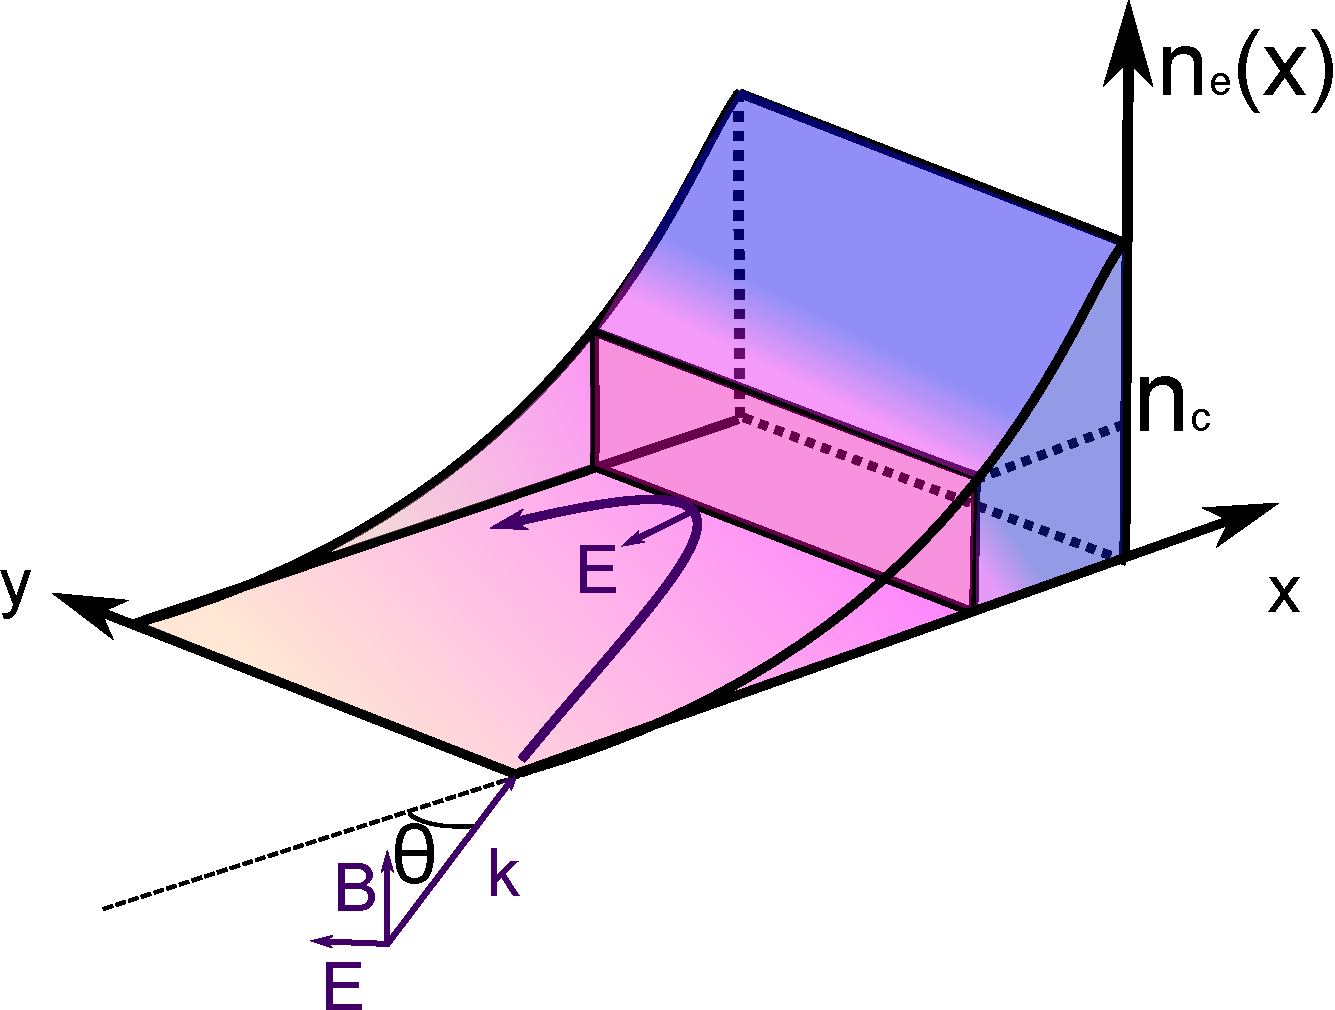
\includegraphics[width =10cm]{../chapitre1/images/gradient.pdf}\\
\caption{\label{fig:gradient} Artistic representation of resonant absorption for a 1-dimensional electron density distribution $n_e(x)$. $\g{k}$ is the incident wave vector and $\theta$ is the incident angle. The field is reflected at the critical surface $n_c$, which coincides with purely normal $\g{E}$ component. This illustration is largely inspired by Figure 2.5 found in~\cite{theseAnto}.}
\end{center}
\end{figure}

\noindent The geometrical representation of a wave propagating in a density plasma, illustrated by Fig~\ref{fig:gradient}, becomes wrong for a short scale length $L$ because the underlying hypotheses behind this representation is that $L >> \lambda$ where $\lambda$ is the driving laser wavelength. Indeed, a representation of an optical wave with $\vec{k}$ changing direction while propagating along $x$ is a geometrical optics representation driven by the eikonal equation \cite{LandauLip}, or in other words the Fermat Principle, and we can write:

\begin{equation}
n(x) \sin\theta(x) = constant
\end{equation}

\noindent That is to say in our case for a propagating wave of frequency $\omega$:

\begin{equation}
(1 - \frac{\omega_p(x)^2}{\omega^2})^{1/2}\sin\theta(x) = \sin(\theta_0)
\end{equation}

\noindent where $\theta$ is expected to increase with x, since $\g{k}$ is directed towards a zone of lower index. In this case, the wave would be refracted by the underdense plasma before it could reach the critical density $n_c$. \\

\noindent This shows that the geometrical approach is incorrect and that propagation in the underdense part  of the plasma, when $L$ is comparable to $\lambda$, needs to be treated using wave equations ~\ref{eq:RAequations}. However, the mental representation given in Fig~\ref{fig:gradient} is still relevant as shown by Freidberg et al. \cite{freidberg1972resonant} who integrated the system of equations ~\ref{eq:RAequations2} for a magnetic field having the form:
$$
B = B_z(x)e^{-i(\omega t - k_y y)}
$$

\noindent where $k_y = \frac{\omega}{c}\sin\theta$ is independent of $x$. The solution in the case of a linear density gradient increasing from $0$ to the critical density is evanescent for $E_y$. This absorption behavior is optimal for a given angle and gradient length ($\theta = 23^{\circ}$ for $L = 1.6 \lambda$). The $E_y$ component of the electric field is rigorously equal to zero at the critical surface while the $E_x$ component of the electric field significantly increases. Therefore: the geometrical representation given in Fig~\ref{fig:gradient} appears correct if instead of picturing the $\g{k}$ vector turning during the propagation, we impose $\theta$ to be constant at all time and instead picture the evanescent $E_y$ component of the electric field.
This singular behavior is associated with a strong coupling of $E_x$ with plasma waves at the critical surface and is responsible for collisionless conversion of the laser energy into electronic kinetic motion~\cite{freidberg1972resonant}.

\noindent The important remark to make about resonant absorption is that the description of a neutral plasma remains valid as long as the scaling law given in Eq.~\ref{eq:Poisson} holds true. In particular, for a plasma at critical density, this implies:
$$
L_0 >> \frac{V_{osc}}{\omega_0}\approx \lambda_0/6
$$

\noindent The numerical estimate is done for a typical electric field of $a_0 = 1$ at $\lambda_0 = 800\,\mathrm{nm}$. In the physical mechanism we consider, the plasma length typically scales as a fraction of the laser wavelength, which is why  a ``Brunel'' absorption model, as presented hereafter, is applicable.






\section{Brunel absorption mechanism}
\label{section:Brunel absorption mechanism}

Brunel's absorption mechanism is crucial in order to understand how the laser beam reflecting off the critical surface can transfer its energy to the plasma without penetrating it. Indeed, up until Brunel's milestone article in 1987 \cite{Brunel1987}, absorption of a short laser pulse ($\mathrm{CO}_2$ lasers with picosecond durations  at the time) by overdense plasmas was mainly attributed to resonant absorption \cite{freidberg1972resonant}. \\

\noindent In Brunel's model, the electrons at the plasma mirror surface respond to the incident laser electric field in such a way that the plasma is no longer considered neutral. At different phase of the driving laser, surface electrons are accelerated towards vacuum following different trajectories, while the much heavier ions remain static. This creates a charge separation field which tends to pull electrons back towards the plasma. As the laser field changes sign, it adds to the ion static field and electrons accelerated in the direction of plasma bulk gain sufficient energy to cross the critical surface and therefore escape the laser influence. As they cross the critical surface with accumulated kinetic energy and "\textit{(...) since the field is null inside, one can see that the kinetic energy given to the particles that reenter the plasma is lost}(Brunel,1987\cite{Brunel1987})", or in other words the laser transfers its energy to the plasma, justifying the term "absorption".

\subsection{Modeling}

A 1-dimensional approach allows one to get an analytical expression of the electron trajectories for a given incident laser field $E_L(t)$ only dependent on time $t$ and defined at the surface of the plasma. We therefore project the electron equation of motion onto the $x$ direction of space and impose $v_y=v_z = 0$ such that:
\begin{equation}
\frac{d(\gamma v_x)}{dt} = -e\underbrace{(\g{E}_I+\g{E}_R).\g{u}_x}_{\mbox{reflection}} - e\underbrace{(v_y B_z - v_z B_y)}_{=0}
\end{equation}

\noindent where $E_I$ and $E_R$ are the incident and reflected fields at the plasma surface. The laser field strength results from their constructive interference such that $E_L(t) = 2E_I(t)\sin\theta$ with the trivial assumption that $|E_I| = |E_R|$.


\noindent Electrons are accelerated away from the critical surface into vacuum creating a space charge field due to the static ions. In result, this space charge field will screen the driving laser field. To account for this screening, we impose the electric field to be rigorously equal to zero at the critical density surface and inside the bulk of the plasma.


\begin{minipage}{0.5\textwidth}
\begin{figure}[H]
\centering
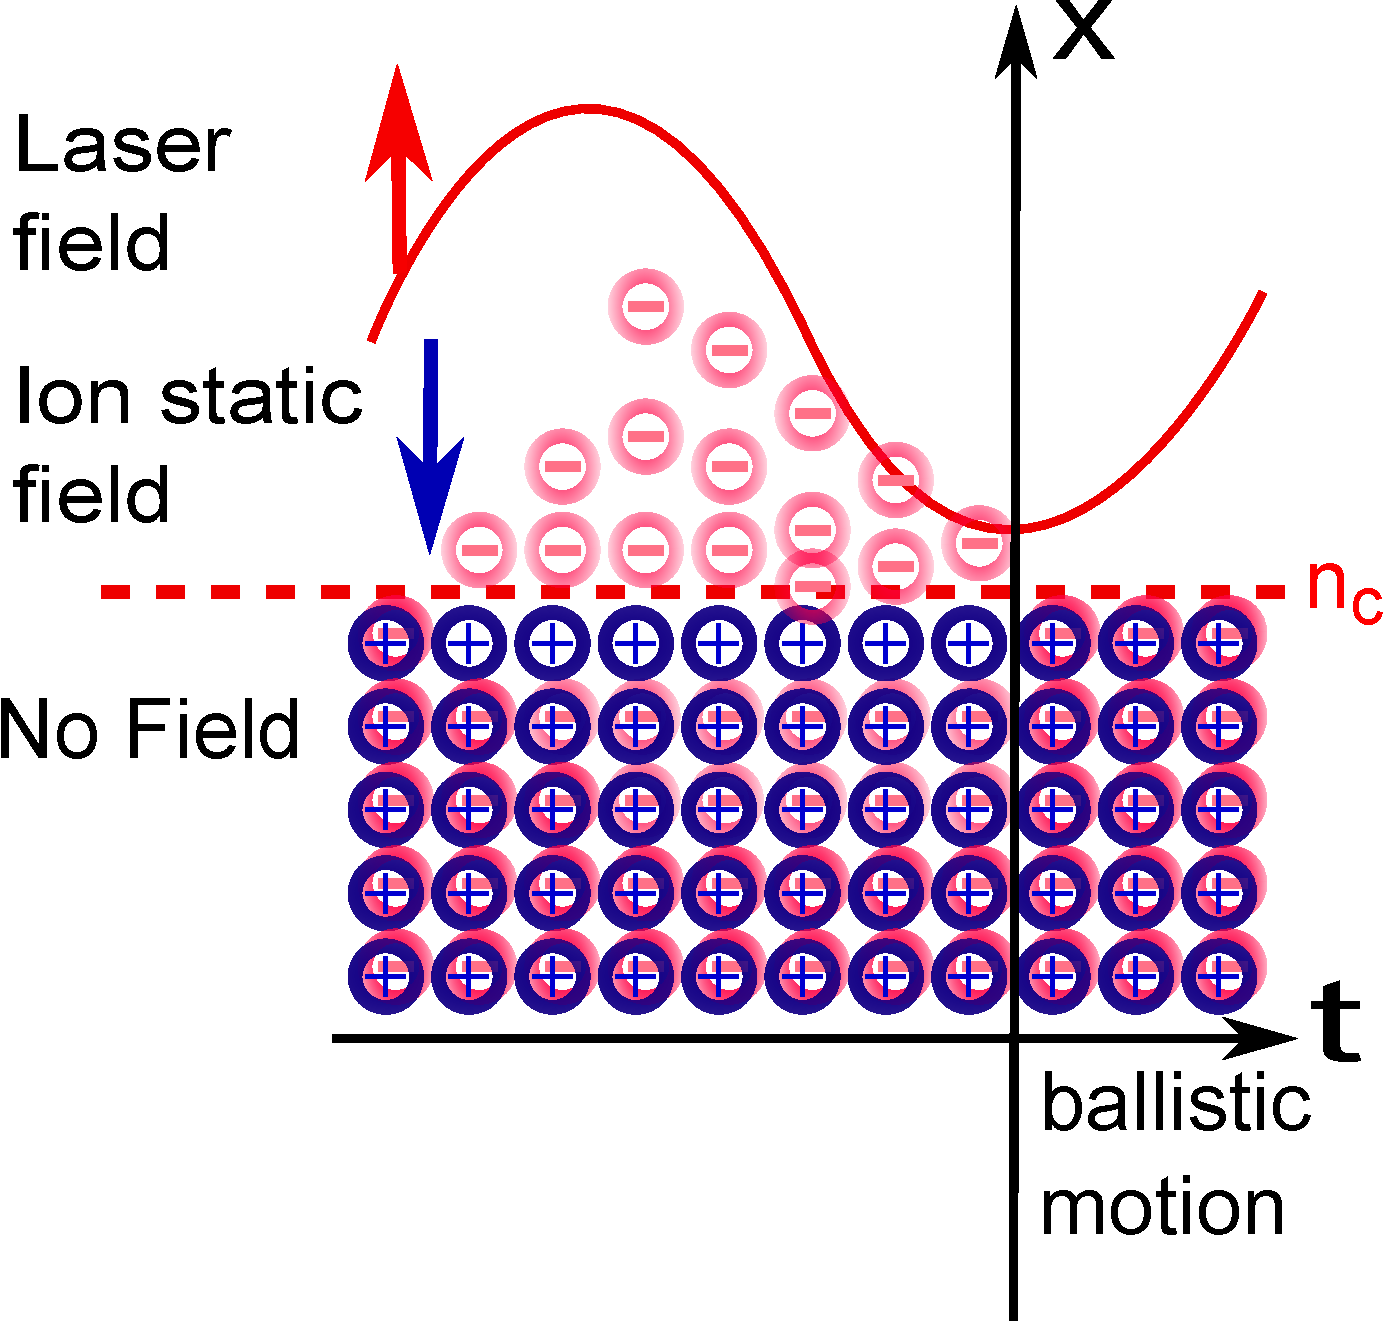
\includegraphics[width =5cm]{../chapitre1/images/BrunelElectrons.pdf}\\
\end{figure}
\end{minipage} \hfill
\begin{minipage}{0.45\textwidth}
Relativistic equation of motion without magnetic field for the $i$th electron born at time $t_i$:
\begin{subequations}
\label{eq:BrunelEqMotion}
\begin{align}[left = \empheqlbrace\,]
   E_i(t) = E_L(t) - E_L(t_i) \\
   \frac{d\gamma_iv_i}{dt} = -eE_i(t)
\end{align}
\label{eq:BrunelEquationMotion}
\end{subequations}
\end{minipage}
\begin{minipage}{0.5\textwidth}
\end{minipage}

\noindent The system of Eq.~\ref{eq:BrunelEqMotion} applies only to vacuum electrons located above the initial critical density surface (represented by the red dotted line).  Note that in this case, the critical surface is located at a constant position $x_c$ in time. This assumption is no longer true for highly relativistic interactions \cite{TheseHenri} and the motion of the critical surface has to be taken into account. This is done in particular in the work of Gonoskov\cite{gonoskov2011ultrarelativistic}. The principle of superposition allows one to add the contribution of the laser field, independent of the position because the electron propagation paths are much shorter than the driving laser wavelength, and the electrostatic field resulting from charge separation. The latter is given by the Poisson equation :


\begin{equation}
\nabla^2 \phi(x,y,z,t) = \frac{\rho(x,y,z,t)}{\epsilon_0}
\end{equation}

\noindent In three dimensions, the analytical solution is written:
$$
\phi(x,y,z,t) =  \frac{1}{\epsilon_0}\int_{\Omega}\rho(x',y',z',t)G(x-x',y-y',z-z')dx'dy'dz'
$$

\noindent where $G$  is the Green function derived in Appendix ~\ref{ch:Green function}  and $\Omega$ the charged region of space. 
In one-dimension, the Green function is defined by $G(r) = -\frac{1}{2}|r|$ such that we have, with $\rho$ defined as a linear charge density:

\begin{align}
\label{eq:fieldDerivation}
E_P(x) = -\partial_x\phi & =  \frac{1}{2\epsilon_0}\partial_x[\int_{\mathbb{R}}\rho(x')|x-x'|dx'] \\
                                   & =  \frac{1}{2\epsilon_0}[\int_{-\infty}^{x}\rho(x')dx'-\int_{x}^{\infty}\rho(x')dx']\\
                                   & =  -\frac{1}{\epsilon_0}[\int_{x}^{\infty}\rho(x')dx']=  -\frac{Q_{x'>x}}{\epsilon_0} \label{eq:fieldDerivation3}
\end{align}
\noindent where $Q_{x'>x}$ is the total charge integrated over $x'>x$.
\noindent Note that the one-dimension model holds true as long as the electrons are "close" to the critical surface or in other words that the lateral dimension of the charge distribution is much greater than its longitudinal dimension. The equation of motion is the result of two simple hypotheses:
(i) The electric field felt by the $i^{th}$ electron is the superposition of the laser field and the charge separation field as expressed in Eq.~\ref{eq:LaserFieldEquations1}, (ii) this field is rigorously equal to zero for $t = t_i^{-}$ at the beginning of motion.


\begin{subequations}
\begin{align}[left = \empheqlbrace\,]
&E_i(t) = E_P(x_i(t)) + E_L(t)\label{eq:LaserFieldEquations1} \\
&0= E_P(x_i(t_i)) + E_L(t_i)\label{eq:LaserFieldEquations2}
\end{align}
\label{eq:LaserFieldEquations}
\end{subequations}


\noindent We subtract ~\ref{eq:LaserFieldEquations2} from ~\ref{eq:LaserFieldEquations1} and note that because of Eq.~\ref{eq:fieldDerivation3}, if we impose that the electron trajectories do not cross, we have $E_P(x_i(t)) = E_P(x_i(t_i))$ at all time such that:

\begin{equation}
E_i(t) = E_L(t) - E_L(t_i)
\end{equation}

\subsection{Physical interpretation}

With Eq.~\ref{eq:BrunelEquationMotion} we can plot the electron trajectories in Fig~\ref{fig:BrunelTrajectories}: every laser period, a bunch of electrons propagates into the neutral dense plasma with non-negligible kinetic energy. This accounts for Brunel's absorption and, as we describe in the next section, gives rise to electronic plasma waves responsible for the generation of attosecond pulses~\cite{thaury2010high}.

\begin{figure}[H]
\centering
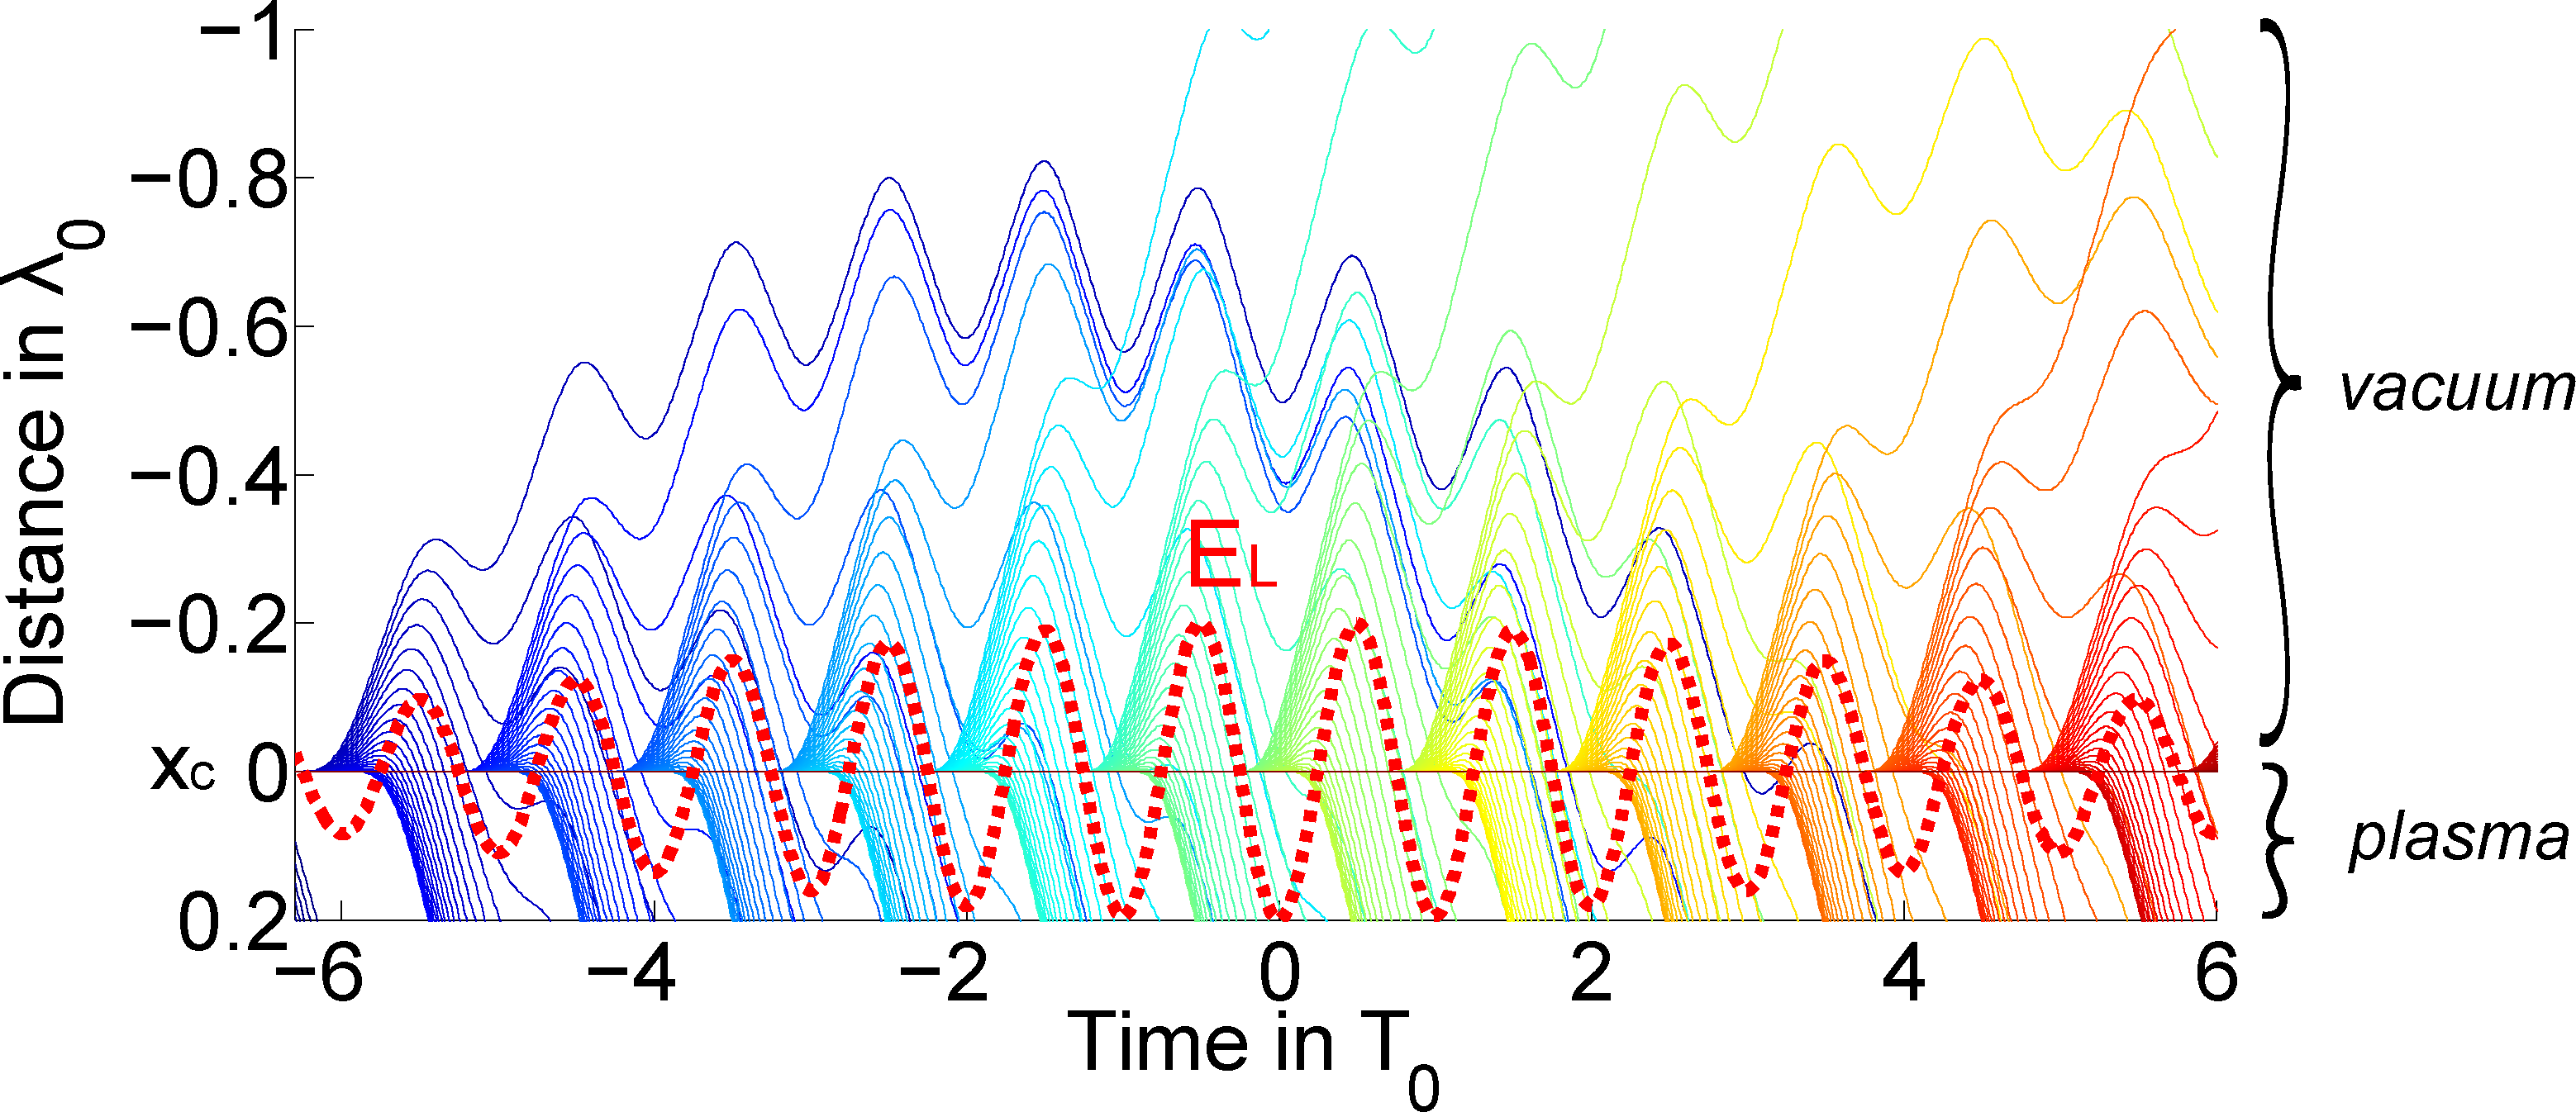
\includegraphics[width =0.8\textwidth]{../chapitre1/images/BrunelTrajectoriesa0=1-20fs.pdf}\\
\caption{\label{fig:BrunelTrajectories}Integration of Brunel's equation for an electric field of intensity $a_0=1$ ($a_0$ convention described in Appendix\ref{ch:Normalisation conventions}) and duration $\tau_{fwhm} = 20 \rm{fs}$. Vacuum is located on the side $x<0$ and a different color scale is used for electrons emitted from different laser cycles.}
\end{figure}

\noindent The simple integration performed in Fig~\ref{fig:BrunelTrajectories} shows that some of the electrons oscillate in vacuum during several laser periods. These electrons are not interesting in the scope of this model because of the 1-dimension hypothesis: in reality, the field should be calculated in three dimensions 
where it undergoes a $\propto 1/|r|^2$ decay instead of being constant as it is the case in 1D. What's more, as the laser pulse is reflected from the critical surface, it generates a time-varying interference pattern which can affect significantly the electron's dynamic as will be developed in Chapter~\ref{Laser-electron interaction in vacumm}, where we describe the electrons acceleration from the plasma mirrors.\\

\noindent In conclusion, in Brunel's model, laser absorption is a consequence of surface electrons crossing the critical surface of the plasma as they follow the periodic oscillation of the driving laser pulse. We presented the simple one-dimensional model and observed how bunches of electron periodically escape the field to the overdense plasma region. \\

\noindent Brunel recognized these electrons as " hot electrons", and compared his model with experimental temperature measurement through Bremsstrahlung emission \cite{bach1983intensity,priedhorsky1981hard,enright1979superthermal}.
Note that several recent articles designate Brunel's theory as one which can explain acceleration of electrons from solid density target towards vacuum. This shortcoming is an extensive interpretation of the term "hot electrons" where electrons escape the target. In Brunels article, the term``hot electron'' refers to the suprathermal tail of a Maxwell-Boltzmann distribution. 
However, using Brunel's model, we can explain the generation of harmonics occurring in the overdense part of the plasma as we describe hereafter.




\section{Harmonic response of an overdense plasma}
\label{section:Harmonic plasma response to Brunel electrons}

One of the great advantages of Brunel's model is to provide a simple equation for the periodic motion of the electrons driven by the laser at the plasma surface. When the returning electrons cross the critical density, their crossing trajectories define an electronic perturbation propagating in the overdense plasma and generating plasma waves in its wake \cite{TheseCedric,TheseArnaud,Thaury2007}. This gives rise to harmonic generation. We will describe the nature of this perturbation and how it relates to the temporal properties of the harmonic emission in Chapter~\ref{chapter:Properties of attosecond pulses emitted using plasma mirrors}. In this Chapter, we focus solely on the response of a plasma to an arbitrary electronic density perturbation.



\subsection{Plasma perturbative approach}
\label{subsection:Plasma perturbative approach}

Let's start with the simple case of a static cold plasma of density $n_e(r,t)$ and study its response to a perturbation. We start with the system of equations:

\begin{equation}
  \left\{
      \begin{aligned}
     &m_e \frac{d(\gamma v(r,t))}{dt} = -e E(r,t) - e v(r,t)\times B(r,t) \\
     &\nabla E =  \frac{\rho}{\epsilon_0}\\
    & \partial_t n + \nabla(nv) = 0
      \end{aligned}
    \right.
\label{eq:PlasmonEquation}
\end{equation}



\noindent The density of the fully ionized plasma is defined such that the plasma is neutral at $t < 0$. In addition, we make the strong hypothesis that the heavier ions do not move, leading to $n_i(r,t) = n_{i0}$. This implies:


\begin{equation}
  \left\{
      \begin{aligned}
     &\rho(r,t) = Z e n_{i0} - e  n_e(r,t)\\
     &m = m_e\\
    &v(r,t) = v_e(r,t)\\
      \end{aligned}
    \right.
\label{eq:Parameters}
\end{equation}

\noindent We also renormalize the variables in the following way (we define $Z=1$ to simplify the notations of the system):

\begin{equation}
  \left\{
      \begin{aligned}
     &\bar{t} = \omega_0 t\\
     &\bar{v} = v/c\\
     &\bar{r} = \frac{2\pi}{\lambda_0 }r\\  
     & \bar{n} = \frac{n}{n_{e0}} 
     & \bar{\rho} = \frac{\rho}{e n_{e0}} = 1 - \bar{n}
      \end{aligned}
    \right.
\end{equation}

\noindent where $n_{e0}$ is the electron density for $t<0$.
In the case of a classical equation of motion ($\gamma = 1$,$v\times B = 0$) for a charged particle of velocity $v$, Eq.~\ref{eq:PlasmonEquation} leads to the system of equations 
~\ref{eq:system}. The corresponding dimensionless equation is given by Eq.~\ref{eq:systemAD} and will be used to describe the plasma's dynamical response to a perturbation.



\begin{multicols}{2}

\begin{subequations}
\label{eq:system}
\begin{align}[left = \empheqlbrace\,]
  &\frac{d n_e}{dt} = - n_e\nabla(v_e)  \label{eq:system1}\\
  &\frac{d( \nabla v(r,t))}{dt} = \frac{-e \rho(r,t)}{m_e \epsilon_0} \label{eq:system2}
\end{align}
\end{subequations}
\begin{subequations}
\label{eq:systemAD}
\begin{align}[left = \empheqlbrace\,]
   \frac{d \bar{n}}{d\bar{t}} = - \bar{n}\nabla_{\bar{r}}(\bar{v})   \label{eq:systemAD1}\\
   \frac{d( \nabla_{\bar{r}} \bar{v}(r,t))}{d\bar{t}} =  \bar{n}(r,t)-1 \label{eq:systemAD2}
\end{align}
\end{subequations}
\end{multicols}






\begin{multicols}{2}
\mbox{Where we pose:}
$$
\frac{e^2 n_{e0}}{m_e\omega_0^2 \epsilon_0} = 1 
$$

\mbox{And by definition:}
$$
\lambda_0= \frac{2 \pi c}{\omega_0}
$$
\end{multicols}

\noindent We obtain a system of differential equations for variables $\bar{n}$ and $\nabla \bar{v}$. One can consider the two-dimensional vector 
$$
X = 
 \left( \begin{array}{c}
\bar{n}(r,t) \\
\nabla_{\bar{r}} \bar{v} \end{array} \right)
$$

\noindent We have according to equations ~\ref{eq:systemAD}
\begin{equation}
  \left\{
      \begin{aligned}
     & \frac{d X}{d\bar{t}} = f(X) \\
     & f(x,y) = (-x y, x-1)
      \end{aligned}
    \right.
    \label{eq:systemNL}
\end{equation}

\noindent Looking at Eq.~\ref{eq:systemAD}, the system is obviously stationary for ($\bar{n} = 1$, $\nabla_{\bar{r}} \bar{v} = 0$), which corresponds to a neutral plasma at rest.
This system can be linearized to the first order by calculating the Jacobian matrix of function $f$ around $(\bar{n} = 1 , \nabla_{\bar{r}} \bar{v} = 0)$. The resulting system of equations is:

\begin{equation}
  \left\{
      \begin{aligned}
     \frac{dX}{dt} = 
 \left( \begin{array}{cc}
0 & -1\\
1 &  0  \end{array} \right)X
      \end{aligned}
    \right.
\label{eq:systemL}
\end{equation}

\noindent We recognize here the equation of a harmonic oscillator \cite{thaury2010high,chen1985acceleration} when linearizing the system in Eq.~\ref{eq:PlasmonEquation} around its stationary solution. In Fig~\ref{fig:PhasePortrait-nonRelativiste} we compare the phase portrait resulting from the integration of Eq.~\ref{eq:systemNL} with its linearized system described by Eq.~\ref{eq:systemL}. In the latter case, we observe a periodic behavior of period $\bar{T} = 1$ in the response to an initial perturbation which means that the plasma oscillates at frequency:


$$
\omega_p = \sqrt{\frac{n_{e0}e^2}{m_e\epsilon_0}}
$$


\noindent High-harmonic generation is due to this resonant plasma response to an initial perturbation, which locally follows Eq.~\ref{eq:systemAD}. We integrated this equation and show the result on a phase plot in Fig~\ref{fig:PhasePortrait-nonRelativiste}, where we also see that the linearized integration is a good approximation of the plasma response. In practice, the plasma is perturbed by a peak of density propagating throughout the density gradient at relativistic velocity $v_p$ and of density several times $n_c$ \cite{thaury2010high,TheseArnaud}.

\begin{figure}[H]
\centering
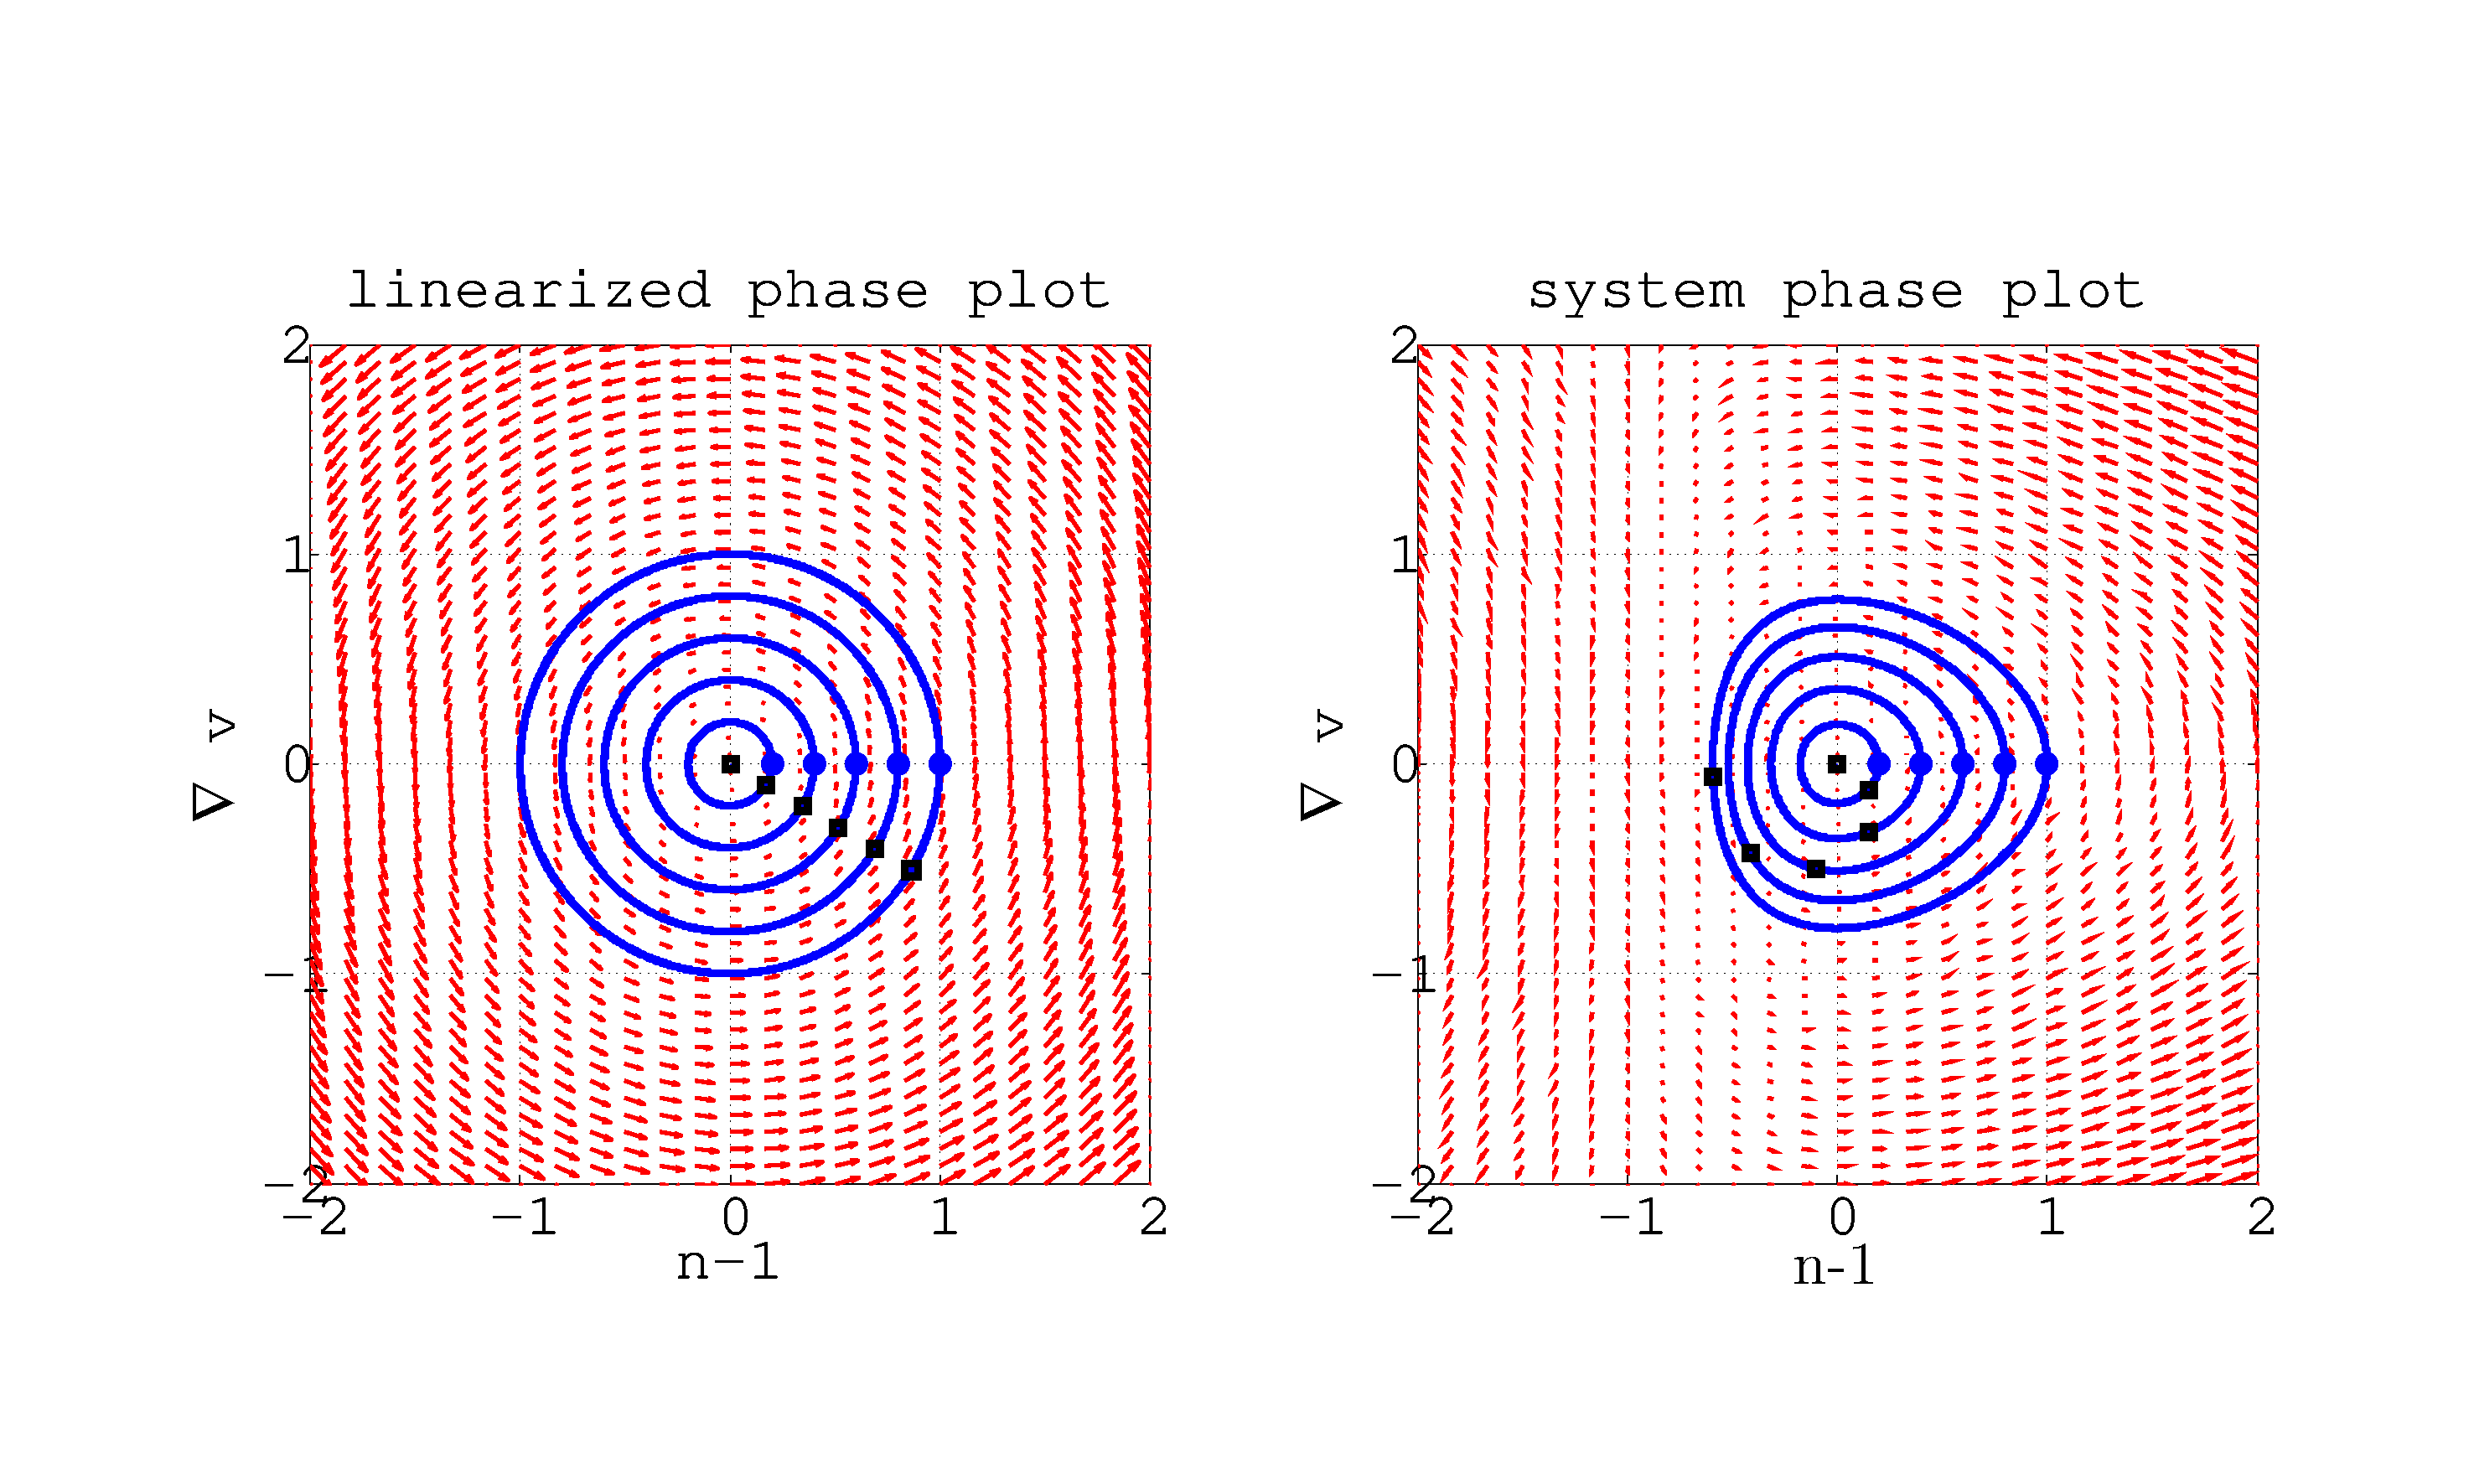
\includegraphics[width =\textwidth]{../chapitre1/images/PhasePortrait-nonRelativiste.pdf}\\
\caption{\label{fig:PhasePortrait-nonRelativiste}Phase plot comparison between the system of equations~\ref{eq:PlasmonEquation} (right) and 
its linearized equivalent (left). The trajectories of $\delta \bar{n} = \bar{n}-1$ and $\nabla\bar{v}$ are integrated and represented for initials perturbation represented by solid circles from $\bar{t} = 0$ to $\bar{t}=100$. Final positions are marked with black solid squares.}
\end{figure}

\noindent So far, the integration has to be done ``locally'', which is equivalent to assuming that the plasma is homogeneous. High inhomogeneities make the integration very challenging and can influence drastically the plasma response to a perturbation as discussed in~\ref{Landau damping in an inhomogeneous plasma}.


\subsection{Coherent Wake Emission}\label{subsubsection:Collective response of density gradient}
\label{subsection:Collective response of density gradient}\label{subsubsection:Collective response of density gradient}

We just described the local electronic response to a perturbation. When the plasma forms at the surface of the solid target, it can not be considered homogeneous as a result of thermodynamical expansion \cite{Kruer1988}.
There, the plasma density is commonly described by a decreasing exponential \cite{kruer1988physics,mora2003plasma} from homogeneous plasma of density $n_{max}$ at position $x_{max}$ to zero density in vacuum as expressed in Eq.~\ref{eq:DensityGradient}:
\begin{equation}
  \left\{
      \begin{aligned}
&\bar{n}_e(x,t) = e^{-(x-x_c)/L} \ \ \rm{for} \ \ x > x_{max}  \\
&\bar{n}_e(x,t) = \frac{n_{max}}{n_c} \ \ \rm{for} \ \ x \le x_{max}
      \end{aligned}
    \right.
\label{eq:DensityGradient}
\end{equation}

\noindent where $n_c$ denotes the critical density at position $x_c$. Vacuum is located at $x>0$


\begin{figure}[H]
\centering
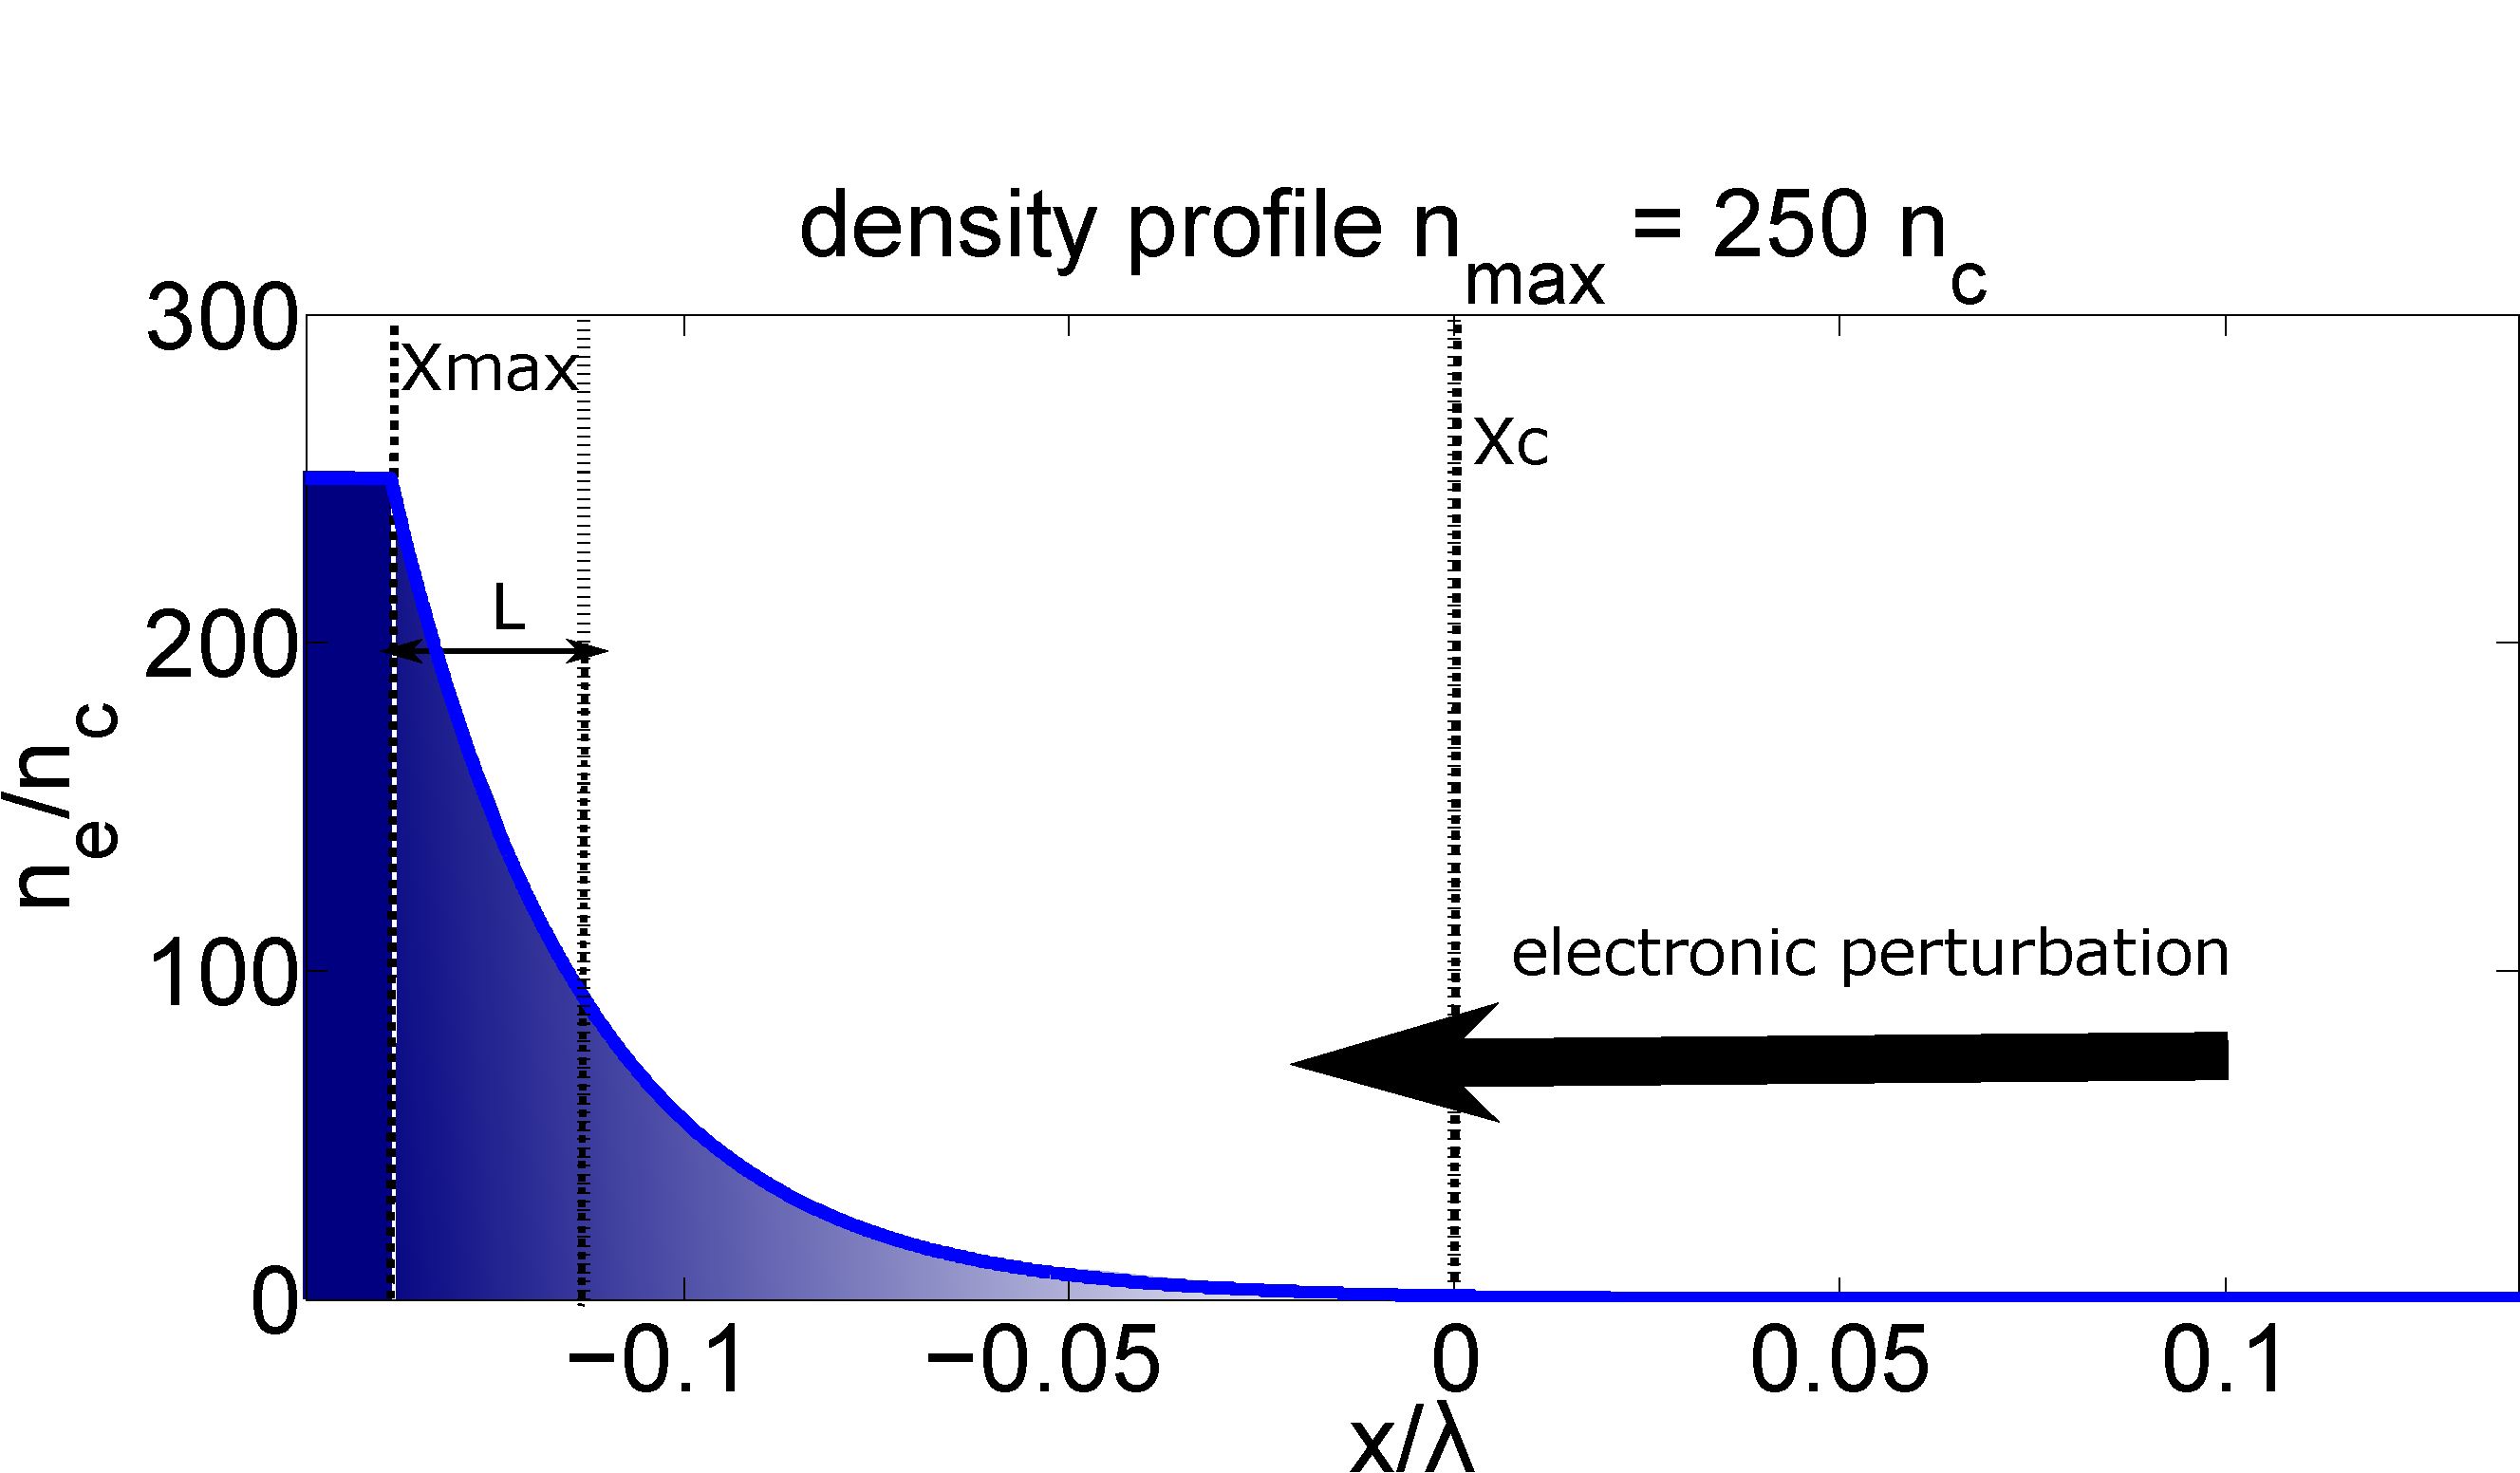
\includegraphics[width =0.6\textwidth]{../chapitre1/images/densityProfil.pdf}\\
\caption{\label{fig:Density Gradient}Density gradient representation defined by Eq.~\ref{eq:DensityGradient}, $L = \lambda / 40$ and $n_{max} = 250n_c$}
\end{figure}



\noindent Let's now consider a perturbation of the electronic density $\Delta_n$ propagating at a speed $v_p$ from $x = 0$ at $t = 0$ towards the bulk plasma. The perturbation reaches the coordinate $x$ at time $t = \frac{x}{v_p}$. We can therefore write in the linearized approximation derived in \ref{subsection:Plasma perturbative approach}:

\begin{equation}
  \left\{
      \begin{aligned}
&\delta\bar{n}_e(x,t) = \Delta_n cos(\omega_p(x) (t-\frac{x}{v_p})) \ \ \  \mbox{for} \ \ \  t \ge \frac{x}{v_p}\\
&\delta \bar{n}_e(x,t) = 0 \ \ \ \mbox{for} \ \ \  t < \frac{x}{v_p}
      \end{aligned}
    \right.
\label{eq:DensityPerturbation}
\end{equation}

\noindent with 
$$
\omega_p(x) = \sqrt{\frac{n_{c}e^2}{m_e\epsilon_0}} \sqrt{\bar{n}_e(x)}= \omega_0 \sqrt{\bar{n}_e(x)}
$$

\noindent where $\bar{n}_e$ is the normalized electronic density defined in Eq.~\ref{eq:systemAD}.\\

\noindent We illustrate Equations~\ref{eq:DensityPerturbation} in Fig~\ref{fig:CWE_illustration} where we represent over time the evolution of the plasma perturbation for plasma scale lengths of respectively $L = \lambda/40$ and $L=\lambda/15$ for an arbitrary density of $n_{max} = 250 n_{c}$. The case $\lambda/15$ shows that for longer gradients, the perturbation has no time to propagate up to the maximum density before the end of an optical cycle. This explains why plasma waves (and therefore harmonic emission) is only efficient for short plasma scale lengths~\cite{thaury2010high,TheseCedric,theseAnto,TheseArnaud}.

\begin{figure}[H]
\centering
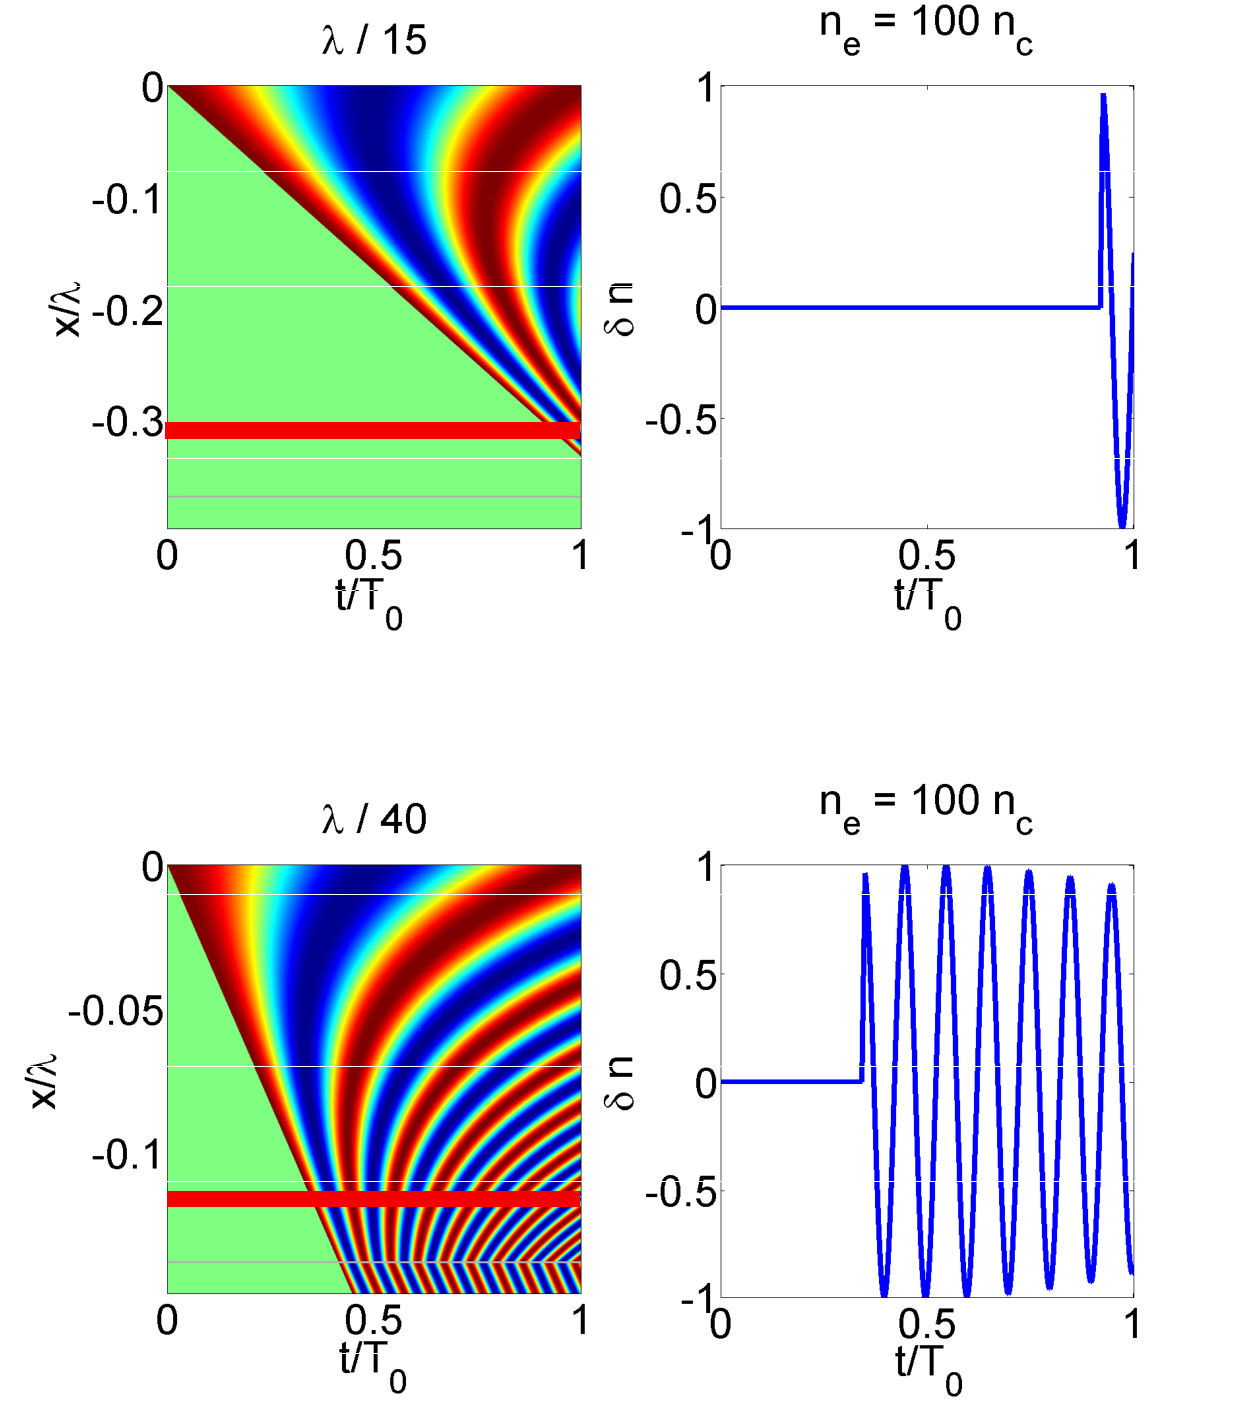
\includegraphics[width =0.6\textwidth]{../chapitre1/images/CWE_illustration.pdf}\\
\caption{\label{fig:CWE_illustration} Representation of plasma oscillations over one laser period for gradients with $L = \lambda/15$ and $L = \lambda/40$, where $n_{max} = 250n_c$. The position where $n_e = 100 n_c$ is represented by a solid red line on the left-hand-side figures, and the corresponding plasma oscillation is plotted on the right-hand-side figure}
\end{figure}


\noindent The link to the generation of high order harmonics is now quite straightforward.
Indeed, since we know that a charge in motion radiates, it follows that plasma waves result in electromagnetic radiation. This emission can be evaluated by integrating the propagation equation applied to the vector potential $\g{A}$ using a Green function formalism (cf \ref{ch:Green function})~\cite{LandauLip}. At a position $\g{r}$ far from the plasma, we calculate the contribution of a volume $\Omega$ from the plasma to the radiation:

\begin{subequations}
\label{eq:SolutionHarmoniquesLongDist}
\begin{align}[left = \empheqlbrace\,]
&\g{A}(\g{r},t) = \frac{\mu_0}{4\pi} \int_{\g{r}' \in \Omega}\frac{\g{j}(\g{r}',t-|\g{r}-\g{r}'|/c)}{|\g{r}-\g{r}'|}d\g{r}' \\
&\phi(\g{r},t) = \frac{-e}{4\pi\epsilon_0} \int_{\g{r}' \in \Omega}\frac{n_e(\g{r}',t-|\g{r}-\g{r}'|/c)}{|\g{r}-\g{r}'|}d\g{r}'\label{eq:SolutionHarmoniquesLongDist2}
\end{align}
\end{subequations}

\noindent where $\g{r}'$ is a position inside the plasma, $n_e$ the electronic density and $\g{j} = -en_e\g{v}_e$ the associated current. Knowing that $\g{E} = -\nabla \phi - \partial_t \g{A}$ and $\g{B} = \nabla\times \g{A}$, we see how currents or plasma waves inside the plasma lead to electromagnetic radiation. If we simplify the problem to the 1-dimension case and inject Eq.~\ref{eq:DensityPerturbation} in Eq.~\ref{eq:SolutionHarmoniquesLongDist2} (where we use the 1-dimension Green function instead), we can write in first approximation for $t\ge t_p(.)$, the time at which perturbations are triggered:

$$
E(x,t) = \frac{e\Delta_n}{2\epsilon_0} \int_{x' \in \Omega}\cos(\omega_p(x')(t-|x-x'|/c-x'/v_p)dx'
$$

\noindent  where we clearly identify the coherent superposition of propagation waves of frequency $\omega_p(x')$. This leads to the following conclusion: 
\begin{itemize}
\item[$\bullet$] The spectrum of the electromagnetic radiation emitted by the plasma contains all possible values of $\omega_p(\g{r}')$ such that \g{Coherent Wake emission} will undergo a spectral cutoff at $\omega_{p,max}$. The field here is expressed as the response to one optical cycle plasma response. This process is repeated every laser period which leads to emission of co-propagating pulses separated by $1/T_0$. In the spectral domain, these pulses interfere constructively for all multiples of the driving laser: this is designated as "High Harmonic Generation" (HHG).
\item[$\bullet$] The time of emission corresponds to the moment where the integral reaches an optimal value.The harmonic emission properties are extensively described in~\cite{thaury2010high}.
\end{itemize}


\subsection{Influence of spatial spreading of the perturbation}


So far, we have considered the perturbation to be a Dirac function in time. Let's see the influence of a temporal spread of the perturbation over an interval $\tau$. 
Given the principle of superposition, we will add the contribution of all resonators born at different time $t_k$: 


\begin{equation}
  \left\{
      \begin{aligned}
&\delta\bar{n}_{e,k}(x,t) = \Delta_k cos(\omega_p(x) (t-t_k)) \ \ \  \mbox{for} \ \ \  t \ge t_k\\
&\delta \bar{n}_e(x,t) =\sum_{k}\delta\bar{n}_{e,k}(x,t) = \sum_{k}\Delta_k \cos(\omega_p(x) (t-t_k))\Pi(t-t_k) 
      \end{aligned}
    \right.
\label{eq:SeveralResonnator}
\end{equation}

\noindent A more accurate way to write this would be to replace the sum by an integral such that:
\begin{equation}
\delta \bar{n}_e(x,t) =\int_{-\infty}^t\Delta(t') \cos(\omega_p(x) (t-t'))dt' .
\end{equation}

\noindent Without developing further, it clearly appears that when $\Delta (t')$ extends over $1/\omega_p(x)$, the integral tends to zero which means the perturbation no longer inefficiently stimulates the plasma. We calculate that the perturbation should verify $\tau << 100-200\,\mathrm{as}$ for harmonics of order from $10$ to $20$. 

\subsection{Landau damping in a homogeneous plasma}\label{Landau damping in an inhomogeneous plasma}

So far, we only use the result derived in~\ref{subsection:Plasma perturbative approach} to describe the global plasma response to a perturbation, which means each infinitesimal portion of the plasma is locally homogeneous. In addition, the absence of dissipative term in the system of equations~\ref{eq:systemNL} ultimately leads the system to oscillate infinitely. However, this representation becomes incorrect for strong inhomogeneities and one should turn to a fluid equation of motion \cite{mora2011introduction} as described in Appendix~\ref{ch:Normalisation conventions}. The dynamics of the system are therefore described by the collisionless, non-magnetic linearized Vlasov equation~\cite{vlasov1945theory}:

\begin{equation}
\label{eq:Vlasov}
  \left\{
      \begin{aligned}
     &\partial_{t} f_e + v_e \nabla_{\g{r}} f_e + F(f_e).\nabla_{v}f_{e0} = 0\\
     & F(v_e) = \frac{e}{m_e}\nabla \phi\\
      \end{aligned}
    \right.
\end{equation}

\noindent where $\phi$ is defined by the relation:
\begin{equation}
\nabla^2 \phi = -\frac{e}{\epsilon_0}\int_{\g{v}\in \mathbb{R}}f_{e}(\g{r},\g{v},t)d\g{v}
\end{equation}


\noindent This equation describes the dynamical evolution of the electronic distribution $f_e(r,v,t)$ given an homogeneous initial distribution $f_{e0}(v)$  at $t=0$. The absence of collisional term in this equation makes it time-reversible. However, Landau derived an exact solution for this equation in 1946 \cite{landau1946vibrations}, highlighting the non-intuitive behavior of plasma waves as they respond to an initial perturbation: the solution undergoes an irreversible evolution. Over time, plasma oscillations will dissipate $\propto e^{-\nu t}$ where $\nu$ is called the damping factor.

\noindent The solution was derived using plane wave decomposition with $\g{k}$ as the wave vector, for a perturbation around the non-perturbed distribution $f_{e0}$ (taken to be equal to a Maxwellian distribution):

\begin{subequations}
\label{eq:SolutionHarmoniques}
\begin{align}[left = \empheqlbrace\,]
&f_{e0}(\g{v}) + \int f_{e1}(\g{v},\g{k},0)e^{i\g{k}\g{r}}\label{eq:SolutionHarmoniques1}\\
&f_{e0}(\g{v}) + \int f_{e1}(\g{v},\g{k},t)e^{i\g{k}\g{r}}\label{eq:SolutionHarmoniques2}
\end{align}
\end{subequations}


\noindent  Here, \ref{eq:SolutionHarmoniques1} refers to the initial perturbation imposed on the system, and ~\ref{eq:SolutionHarmoniques2} the resulting distribution at an arbitrary time of plasma evolution. With this notation, the Poisson equation is:
\begin{equation}
k^2 \phi =  \frac{e}{\epsilon_0}\int_{\g{v}\in \mathbb{R}}f_{e1}(\g{v},\g{k},t)d\g{v}.
\end{equation}


\noindent In the case $k \lambda_D << 1$, where $\lambda_D$ denotes the Debye length defined in Appendix~\ref{ch:Normalisation conventions} a solution is given by the relations~\cite{vlasov1945theory}:

\begin{subequations}
\label{eq:DispertionRelation}
\begin{align}[left = \empheqlbrace\,]
     &\omega^2 = \omega_p^2(1+3k^2\lambda_D^2)\label{eq:DispertionRelation1}\\
     & \nu = \omega \sqrt{\frac{\pi}{8}}\frac{1}{(k\lambda_D)^{3}}e^{-1/(2k^2\lambda_D^2)} \label{eq:DispertionRelation2}
\end{align}
\end{subequations}

\noindent where one clearly identifies, in Eq.~\ref{eq:DispertionRelation1}, a dispersion relation for plasma perturbations inside the plasma. For increasing $k$ values, plasma waves are damped over time. 
In the context of this thesis, only timescales for damping on the order of  the driving laser period $T_0$ are of interest. However, in the worst case scenario ($k\lambda_D\approx 1$) we have:
$$
T_0 \nu \approx 2\sqrt{\frac{\pi}{8}}e^{-1/2} \omega_p T_0  \approx 1.5 \pi \sqrt{\frac{n_{e0}}{n_{c}}}
$$

\noindent This indicates that strong plasma inhomogeneities (relative to the Debye length $\lambda_D$) can be dissipated in a dense plasma on a time scale which compares with the driving laser through Landau damping. In Appendix~\ref{ch:Normalisation conventions}, we derive $\lambda_D$ and evaluate its value for $\lambda_0 = 800$nm, $k_BT_e = 100$eV, leading to:
\begin{equation}
\lambda_D = \sqrt{\frac{n_c}{n_{e0}}}1.78\,\mathrm{nm}
\end{equation}

\noindent The case $k \lambda_D >> 1$ is treated in \cite{landau1946vibrations} but is of no interest here. Note that in the present introduction to Landau damping, the plasma is assumed to have a homogeneous density distribution. However, in the context of this thesis,
the generated plasma distributions on solid targets (before any perturbation) outline strong inhomogeneities where the typical scale length $L$ is a fraction of the driving laser wavelength. As a consequence, we have no certainty that the present derivation of plasma response still applies. 

\subsection{Landau damping in an inhomogeneous plasma}

For very short gradients ($L < \lambda/300$), plasma oscillations undergo strong damping effect as demonstrated by PIC simulations performed in \cite{thaury2010high}. This ultimately results in a significant drop in CWE emission.
Similar to Eq.~\ref{eq:SolutionHarmoniques}, we write the system evolution in the form:

\begin{subequations}
\label{eq:SolutionHarmoniquesNH}
\begin{align}[left = \empheqlbrace\,]
&f_{e0}(\g{r},\g{v}) + f_{e1}(v,r,0)\label{eq:SolutionHarmoniquesNH1}\\
&f_{e0}(\g{r},\g{v}) + f_{e1}(v,r,t)\label{eq:SolutionHarmoniquesNH2}
\end{align}
\end{subequations}

\noindent The linearized Vlasov equation given in~\ref{eq:Vlasov} is affected by this and is now:

\begin{equation}
\label{eq:VlasovNH}
\partial_{t} f_{e1} = \underbrace{-v_e \nabla_{\g{r}} f_{e0} - v_e \nabla_{\g{r}} f_{e1}}_{\text{inhonomogeneity damping}} -  \underbrace{F(f_{e1}).\nabla_{v}f_{e0} - F(f_{e1}).\nabla_{v}f_{e1}}_{\text{thermal damping}}
\end{equation}


\noindent The challenging case of an inhomogeneous plasma has been partially treated in \cite{karpman1974nonlinear,asseo1972effect}, where in the case of strong plasma density inhomogeneities, Laudau damping becomes
important and is quantified by the damping factor:
$$
\alpha = -\frac{\omega^2}{2k^2}\frac{1}{L^2}
$$

\noindent where $L$ is the characteristic variation length which we identify as our gradient scale length. $\alpha T_0^2 >> 1$, where $T_0$ is the driving laser period, corresponds to a highly inhomogeneous case.

\noindent The rigorous analytical resolution of the inhomogeneous case is quite challenging and remains a current field of research. However, PIC simulations should in principle reproduce this damping effect: we compare the plasma response of a gradient density perturbed by an incoming electron bunch propagating at a velocity close to $c$ towards the bulk in the absence of a laser beam. This way, we can only observe a pure plasma wave resulting from the electronic perturbation. In Fig~\ref{figDampingEffect_shortGradient}, the plasma
electronic density fluctuation is represented for respectively $L=\lambda/40$(left) and $L=\lambda/300$(right).
One clearly sees that when the plasma scale length is very short, the electronic plasma waves are quickly damped. In this simulation, the plasma temperature is taken equal to zero. In case of Landau damping, we should 
expect the attenuation to be all the more pronounced as we increase the temperature of the plasma. 


\begin{figure}[H]
\centering
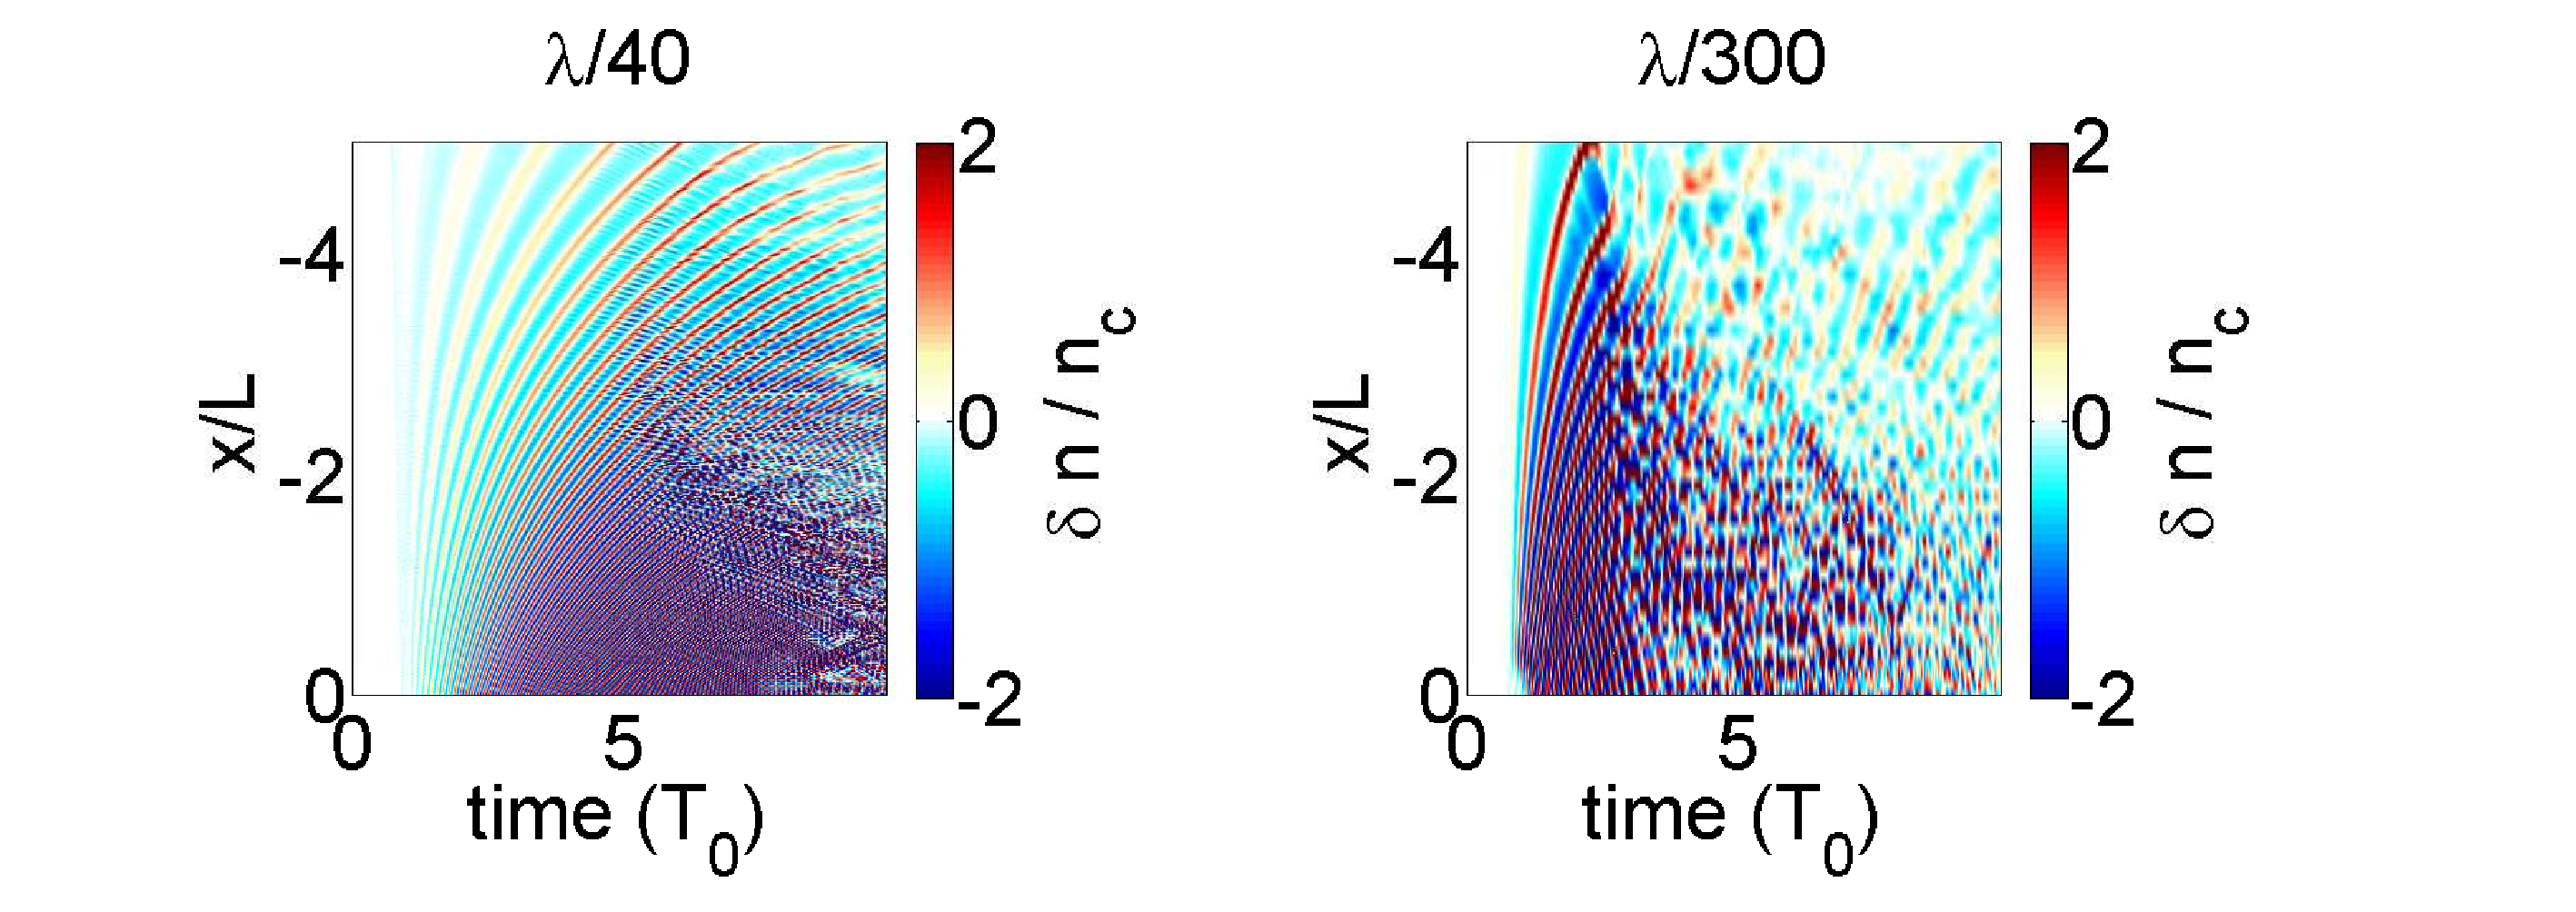
\includegraphics[width =\textwidth]{../chapitre1/images/DampingEffect_shortGradient.pdf}\\
\caption{\label{figDampingEffect_shortGradient}1D pic simulation of plasma oscillations over time triggered by an electronic perturbation. The maximum density is $n_e = 100 n_c$ the gradients are $\lambda /40$ (left) and $\lambda /300$ (right) respectively.
The very short gradient shows damping effect due to strong inhomogeneities of the plasma. The electronic perturbation $\Delta_n = n_c/100$ and propagates at $v_p\approx c$ towards the plasma. The plasma initial temperature is $T_e = 0$ eV}
\end{figure}




\section{Conclusion}

In this chapter, we have gone through the detailed presentation of the different mechanisms involved to understand short plasma scale length response to a femtosecond laser pulse. We presented the resonant absorption model only valid for very long plasma scale lengths by placing it in its historical context, that is to say before high-intensity gradient controlled experiments on solid targets were made possible using contrast cleaning techniques.\\

\noindent For short plasma scale lengths, we showed how the Brunel model provides an accurate representation of the electron motion in presence of a laser field. Brunel electrons are responsible for the emergence of electronic perturbations inside the plasma bulk: we explained in details how these perturbations give birth to plasma waves by solving the harmonic equation of the plasma with given density. Plasma waves in return emit X-UV light every laser cycle. This defines the Coherent Wake Emission mechanism~\cite{thaury2010high,dromey2009tunable,nomura2009attosecond}. \\

\noindent Finally, we have seen how a fluid representation of the plasma is necessary to describe plasma wave damping occurring for very short plasma scale lengths. This is called Landau damping and was confirmed by 1D PIC simulations. We will demonstrate this effect in a gradient-control experiment in Section~\ref{Influence of gradient scale length on harmonic generation}.\\
































